\begin{frame}[parent={cmap:software-testing},hasnext=true,hasprev=true]
\frametitle{Software testing}
\framesubtitle{Definition}
\label{concept:software-testing}

\begin{block:concept}{Definition}
Software testing is the process of operating a system or component under
specified conditions, observing or recording the results, and  making
an evaluation of some aspect of the system or component~\cite{ieee610.12:1990}.
\end{block:concept}

\begin{block:fact}{Software testing is\dots{}}
\begin{itemize}
	\item a verification and validation activity,

	\item important for maintenance, reliability assessment,software process
	improvement, debugging,

	\item a dynamic activity,
	\begin{itemize}
		\item It requires the execution of the program (static analysis is
		not enough)
	\end{itemize}

	\item expensive~\cite{harrold:2000}
\end{itemize}
\end{block:fact}
\end{frame}



\begin{frame}
\frametitle{Software testing}
\framesubtitle{Goal}

\begin{block:fact}{Goal}
\begin{itemize}
	\item The goal of software testing is to detect faults in the product
	under test.
\end{itemize}
\end{block:fact}

\begin{figure}
	\centering
	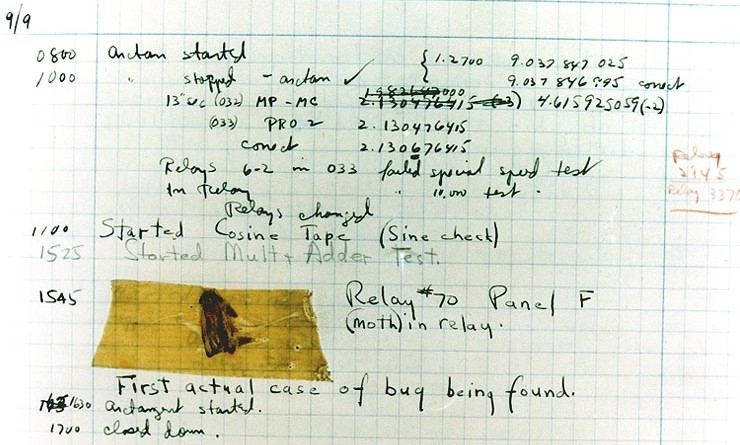
\includegraphics[width=7cm]{first-bug}
	\caption{First detect error (an actual bug).}
\end{figure}
\end{frame}


\begin{frame}
\frametitle{Sofware testing}
\framesubtitle{Main concepts}

\begin{block:fact}{How are faults detected?}
\begin{itemize}
	\item Faults are detected running the software under testing against a set
	of test cases.
\end{itemize}
\end{block:fact}

\begin{block:procedure}{Test case execution}
\begin{enumerate}
	\item Define the input data to be fed to the software under testing.

	\item Run the software.

	\item Check if the result the software produced was the expected one (for
	the given input data).
	\begin{itemize}
		\item If the result is correct, keep defining different input data.

		\item If the result is incorrect, a fault was found! Success!
	\end{itemize}
\end{enumerate}
\end{block:procedure}
\end{frame}



\begin{frame}
\frametitle{Sofware testing}
\framesubtitle{Main concepts}

\begin{block:principle}{Exhaustive testing}
If the software is executed against all possible input data,
any fault will be found!
\end{block:principle}

\begin{block:fact}{Feasibility and computability}
Unfortunately, it is often not possible to run exhaustive testing due to
some computational problems:
\begin{itemize}
	\item the input domain may be so big that it is impossible to run the
	software against it in a reasonable time,

	\item computability (undecidable problems).
\end{itemize}
\end{block:fact}
\end{frame}


\begin{frame}
\frametitle{Software testing}
\framesubtitle{Main concepts}

\begin{block:principle}{Domain partitioning}
Nonetheless, it is possible to partition the input domain and, instead of
using all elements within each partition, just a few ones are selected (and
accepted as a good representation of every element in the set).
\end{block:principle}

\begin{block:fact}{Techniques and criteria}
\begin{itemize}
	\item Test criterion defines rules regarding how a given input domain is
	partitioned.

	\item Such rules, when applied to the software under testing, generates
	test requirements.
	\begin{itemize}
		\item Test requirement is a combination of elements of the program
		under testing that must be satisfied by the execution of a test case.
	\end{itemize}

	\item Test technique defines the rationale and source of information that
	guides the development of test criteria.
\end{itemize}
\end{block:fact}
\end{frame}



\begin{frame}[c]
\frametitle{Software testing concepts}
\framesubtitle{Main concepts}

\begin{figure}
    \centering
    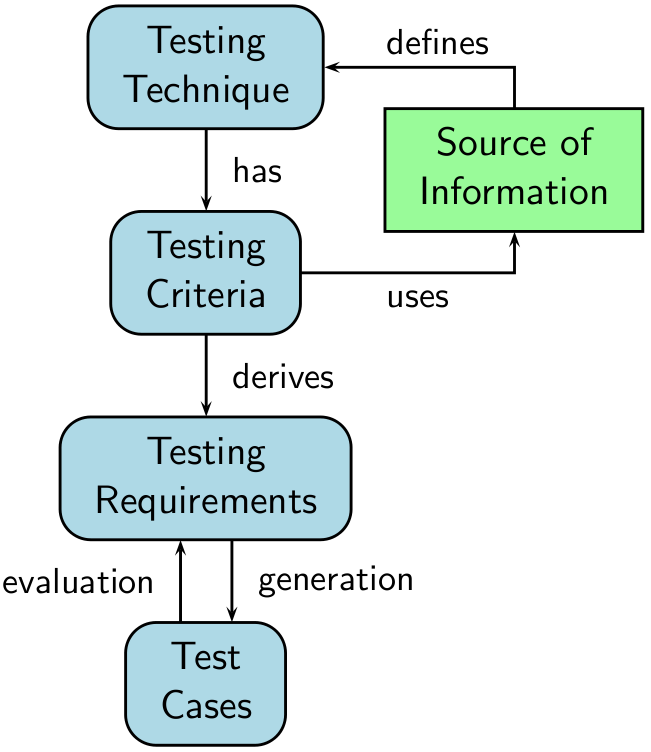
\includegraphics[scale=.3]{software-testing}
\end{figure}
\end{frame}
